\section{The Theory of Compressed Sensing}

We now switch gears and focus on the theory of compressed sensing and group testing, which are the main mathematical tools we use for software testing. We first introduce the key concepts arising in compressed sensing: sparsity, linear measurements, and recovery of sparse active signals. We describe recoverability and efficient algorithms. We then move to Boolean compressed sensing, which is also known in statistics literature as the classical group testing problem \cite{dorfman1943detection, group_testing}. 


\subsection{Search for sparse signals}

There is a great variety of practical problems where we have an unknown vector $\bx$
of large dimensions $N$, which we would like to learn, but it is too expensive to measure all
the coordinates of the vector. The classical application which served as the original motivation
for group testing was testing US army recruits for syphilis during the Second World War. 
Individual blood tests for every one of the large number of recruits were too expensive, 
and statisticians consulting for the US army proposed to take pooled measurements, where 
each test was done on a mixture of blood samples coming from a number of carefully chosen 
recruits. Given enough such pooled tests, and assuming that only a small fraction of the 
recruits had the disease, it was possible to identify the infected recruits.  


In our application to security testing, there is a very large number of individual tokens and 
their small combinations such as pairs and triplets (or patterns as we refer to them). Testing each individual token, pair and 
triplet of tokens through a sanitizer is impractical -- requiring an immense number of calls to the 
sanitizer. However, we know that the vast majority of such patterns is innocuous, 
and only a very small fraction is malicious. 

Compressed sensing suggests to take a reduced set of aggregate measurements of the variable $\bx$,
where each measurement involves a subset of variables $x_i$ together.  For our application of
software testing we would create a string composed of multiple tokens of interest.  For the
army recruit testing problem one would mix the blood samples of multiple soldiers together
in one test-tube and administer the test on the mix.


Given these aggregate measurements where each variable $x_i$ may appear in multiple tests
(i.e., where each test involves a different but typically overlapping subset of indices), we would like to un-mix the
measurements to be able to precisely explain the anomalies at the level of individual tokens,
or individual sick soldiers.  The fact that this is at all possible may seem surprising, but it
is based on very elegant theory building on linear algebra and geometry of polytopes.  An
efficient solution is available using numerical optimization (namely linear programming) which
can recover the true identity of a sparse set of {\em active inputs} from a number of aggregate
measurements which is much smaller than $N$. Applications of similar flavor occur in
other diverse fields such as spectrum estimation, genetic disease testing, and even feature
selection in machine learning. We next describe the mathematical foundations for this exciting
theory.

\subsection{ Linear compressed sensing}

Suppose that  vector $\bx \in \rR^N$ has a small number $K$ of non-zero elements, $K \ll N$.
We denote the number of non-zero elements of $\bx$ using the $\ell_0$-norm notation:
$\Vert \bx \Vert_0 = K$.   We take $M$ aggregate linear measurements $y_i = \ba_i^T \bx$, where
$K < M \ll N$ and aggregate them into a vector $\by = [y_1, ..., y_M]$:
\begin{equation}
\by = A \bx,
\end{equation}
where the matrix $A$ contains vectors $\ba_i$ as rows. Now, given $\by$ and knowing the
measurement matrix $A$, can we hope to recover the unknown
sparse vector $\bx$?  It turns out that if $A$ was chosen properly, and if $\bx$ is sparse
enough, then indeed we can. Furthermore, this recovery can be done by an efficient optimization
procedure, namely linear programming (LP).

First we recall a theorem that allows brute force exact recovery \cite{donoho_pnas}. Define the {\em spark}
$S(A)$ of a matrix $A$ as the minimum number of linearly dependent columns of $A$. This is related to,
but different from rank of the matrix\footnote{For example, it's easy to construct a matrix of rank
$3$, which has two $2$ linearly dependent columns: just take an arbitrary rank-$3$ matrix and
copy one of the columns twice! This matrix has rank $3$ but it's spark is $2$. }. It turns out that
one can recover uniquely sparse vectors which have at most $S(A) / 2$ non-zero entries.

\begin{theorem}
\label{thm:spark}
Suppose that $\Vert \bx \Vert_0 = K < S(A) / 2$. Then there is a unique solution to the
set of equations $\by = A \bx$.
\end{theorem}

This suggests that one can formulate the following optimization problem to find the sparse set of solutions
\begin{equation}
\label{eqn:l0_sparse_recovery}
\min_{\bx} \Vert \bx \Vert_0  ~~\mbox{ s.t. }~~ \by = A \bx
\end{equation}
Now, while the solution of this problem will give us the desired sparse signal (proviso the conditions in
theorem \ref{thm:spark}), the problem has no tractable solution; indeed it is an NP-hard problem \cite{natarajan1995sparse_recovery_complexity}. Astonishingly, under stronger conditions, the solution to this problem can be obtained exactly by a linear
programming (LP) relaxation where we replace the count of non-zeros $\Vert \bx \Vert_0$  by the $\ell_1$-norm
of the vector $\Vert \bx \Vert_1 = \sum_i | x_i|$. The problem becomes:\footnote{This optimization problem can be represented as a linear
program by a standard simple trick of introducing variables $\bx^+$ and $\bx^-$, where $\bx = \bx^+ - \bx^-$,
and $\bx^+, bx^- \ge 0$. }
\begin{equation}
\label{eqn:l1_sparse_recovery}
\min_{\bx} \Vert \bx \Vert_1  ~~\mbox{ s.t. }~~ \by = A \bx
\end{equation}

The conditions in theorem \ref{thm:spark} are not sufficient to guarantee exact recovery of
sparse active inputs using the LP relaxation. However, let us define a relaxed notion of
well-posedness of the matrix $A$ called incoherence. Assume without loss of generality that
the columns of $A$ are normalized to have Euclidean unit norm, i.e., $\Vert A_i \Vert_2 = 1$.  We define the incoherence of $A$ to be:
\begin{equation}
M(A) \triangleq \max_{i \ne j} | A_i^T A_j |
\end{equation}
Using this definition, the following theorem holds:

\begin{theorem}
\label{thm:incoherence}
If $\Vert \bx \Vert_0 \le \frac{ 1 + \frac{1}{M(A)}} {2}$ then the solution of the $\ell_1$-relaxed
problem (\ref{eqn:l1_sparse_recovery}) is also optimal for the combinatorial problem
(\ref{eqn:l0_sparse_recovery}).
\end{theorem}

Note that this does not mean that one can solve the NP-hard problem (\ref{eqn:l0_sparse_recovery})
using LP relaxations in general. This can be done only if the matrix is well-posed, as
specified by the incoherence condition, and if the signal of interest $\bx$ is sparse enough
with respect to $A$.

This condition is sufficient, but not the tightest known condition.
Stronger conditions have been developed based on the so-called Restricted Isometry Property,
\cite{candes2008_RIP} which considers larger subsets of columns of $A$, not just pairs.
However, verifying RIP is just as hard as solving problem (\ref{eqn:l0_sparse_recovery}) in general. In practice, RIP is used for random measurement
matrices $A$, which fortunately can be shown to satisfy the RIP property with high probability. \\


\section{ Boolean compressed sensing}
\label{s:boolean_compressed_sensing}
In many applications we have a very similar problem of having aggregate measurements
of a sparse unknown vector $\bx$, but the measurements may be non-linear.  For the application
to software testing, we will be especially interested in Boolean measurements, where the
vector $\bx$ is binary, and each measurement corresponds to a disjunction of a subset
of entries of $\bx$.  While one would think that recovery of active inputs from
Boolean measurements should be based on very different principles, it turns
out that the core information theoretic issues are closely related, and a very similar linear
programming relaxation can be used for recovery \cite{Malyutov78,MalioutovM2012}.

To set up the notation, we now assume that $\by$, $A$ and $\bx$ are all binary $\{0, 1\}$.
The boolean vector $\bx \in \{0, 1\}^N$, has $K \ll N$ non-zero (faulty) entries.
We will call items $j$ with $x_j = 0$ 'normal'. A pooled measurement $y_i$ is the
Boolean sum (Boolean OR) of $x_j$ in some subset $A_i \subset \{1,..,N\}$, i.e.,
\begin{equation}
y_i = \vee_{j \in A_i} x_j.
\end{equation}
The $M \times N$ measurement matrix $A$ satisfies $A_{ij} = 1$ if item $j$ belongs
to the subset pooled in test $i$. Other entries are $0$. We use the following vector
notation to describe the entire set of $M$ measurements:
\begin{equation*}
\by = A \vee \bx~~~~~~~~
\end{equation*}

\begin{figure}[!thb]
\centering
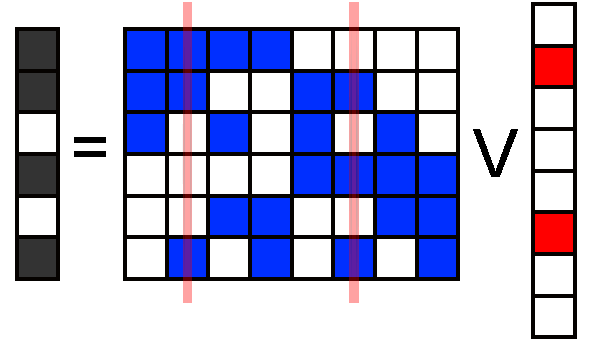
\includegraphics[width=1.5in]{./fig_group_test.pdf}
\caption{  Illustration of a pooled Boolean measurement.}
\label{fig:group_testing}
\end{figure}

It turns out that the story of exact recovery is parallel to the linear case:
if the matrix has well-distributed columns (as captured by the notion of disjunctness as 
defined below) and if the vector is sparse enough, then it can be uniquely recovered from the
Boolean measurements \cite{group_testing}.

\begin{definition}
We call a measurement matrix $\mathbf{A}$ {\em $K$-separating}
if all Boolean sums of subsets of $K$ columns are all distinct.
$\mathbf{A}$ is called {\em $K$-disjunct} if the union of any
$K$ columns does not contain any other column.
\end{definition}

Note that the $K$-separating property for $\mathbf{A}$ is sufficient
to allow exact recovery of $\mathbf{w}$ with up to $K$ nonzero entries
\cite{book2_group_testing}. However, finding the solution would
in general require searching over all $K$-subsets out of $N$. K-disjunctness
is a stronger condition, and allows the recovery using simpler algorithms.

The combinatorial algorithm asks to find the sparsest solution to the
set of Boolean equations which is done by solving the following optimization problem:
\begin{equation}
\label{eq:l0recovery}
	\min \|\mathbf{x}\|_0 \quad {\textrm{such that }}\mathbf{y} = \mathbf{A} \lor \mathbf{x},
\end{equation}

We now describe the LP relaxation for the Boolean sparse recovery problem. While
the problem in (\ref{eq:l0recovery}) looks very similar to the linear one in
(\ref{eqn:l0_sparse_recovery}), the key challenge is that the measurements are not linear. However, they can be represented equivalently by a pair of linear equalities and inequalities.

Let $\mP= \{i | y_i = 1\}$ be the set of measurements $i$ where $y_i$ is positive,
and $\mZ = \{i | y_i = 0\}$ be the set of zero (or negative) tests. Then we can
see that for $i \in \mZ$ we have
\begin{equation}
\mathbf{A}_{\mZ}\mathbf{x} = \mathbf{0}
\end{equation}
For the set of positive measurements, in the Boolean case $1+1 = 1$, while
in the linear case $1 + 1 = 2$, but it is always true that
\begin{equation}
\mathbf{A}_{\mP}\mathbf{x} \ge \mathbf{1}
\end{equation}
These constraints can be incorporated into an equivalent integer program (IP):
\begin{align}
\label{eq:booleanl1min}
	\min\quad &\sum_{j=1}^{n} x_j \\
	\textrm{s.t.\quad} & x_j \in \{0,1\},\,j = 1,\ldots,n\nonumber\\
		& \mathbf{A}_{\mP}\bx \ge \mathbf{1}\nonumber\\
		& \mathbf{A}_{\mZ}\bx = \mathbf{0}.\nonumber
\end{align}
Note that since $x$ is Boolean, the objectives are equivalent (i.e., $\|x\|_0=\sum_i{x_i}$), and yet still, the problem
\eqref{eq:booleanl1min} is NP-hard because of the Boolean integer constraint on the weights. However, relaxing the binary constraints to linear interval constraints, we get a tractable linear program (LP):
\begin{align}
\label{eq:booleanl1minLP}
	\min\quad &\sum_{j=1}^{n} x_j \\
	\textrm{s.t.\quad} & 0\leq x_j \leq 1, \,j = 1,\ldots,n\nonumber\\
		& \mathbf{A}_{\mP}\bx \ge \mathbf{1}\nonumber\\
		& \mathbf{A}_{\mZ}\bx = \mathbf{0}.\nonumber
\end{align}

In \cite{MalioutovM2012} it was shown that if the $A$ matrix is $K$-disjunct, 
then we can recover sparse inputs $\bx$ with at most $K$ non-zero entries using 
the LP in (\ref{eq:booleanl1minLP}).
\begin{theorem}
\label{thm:LP_recovery}
Suppose there exists $\bx^*$ with $K$ nonzero entries and
$\by = \mathbf{A} \lor \bx^*$. If the matrix $\mathbf{A}$ is $K$-disjunct then
LP solution $\hat{\bx}$ in (\ref{eq:booleanl1minLP}) recovers $\bx^*$, i.e. $\hat{\bx} = \bx^*$.
\end{theorem}

This is a sufficient condition, but not necessary. In practice, one can apply
the LP approach even if the LP yields fractional solution, with the help
of randomized rounding or other approaches for mapping to binary numbers.

In practical situations, we typically have noisy measurements.
We consider noise on the $\by$ vector, where some bits can flip from
$0$ to $1$ and vice versa. We represent this by
\begin{equation}
\label{eq:noisyforwardtest}
	\mathbf{y} = (\mathbf{A} \lor \mathbf{x}) \oplus \mathbf{n},
\end{equation}

To extend the LP formulation in the presence of noisy measurements (where $\mathbf{y} = (\mathbf{A} \lor \mathbf{x}) \oplus \mathbf{n}$), we look
for sparse rules that do not match $\by$ exactly, but rather approximate
$\by$ very closely. The corresponding LP formulation is:
\begin{align}
\label{eq:booleanl1minLPslack}
	\min\quad &\sum_{j=1}^{n} x_j + C\sum_{i=1}^{m}\xi_i\\
	\textrm{s.t.\quad} & 0 \le x_j \le 1,\,j = 1,\ldots,n\nonumber\\
		& 0 \le \xi_i \le 1, ~i \in \mP \nonumber\\
		& 0 \le \xi_i, ~i \in \mZ\nonumber\\
		& \mathbf{A}_{\mP}\mathbf{x} + \boldsymbol{\xi}_{\mP} \ge \mathbf{1}\nonumber\\
		& \mathbf{A}_{\mZ}\mathbf{x} = \boldsymbol{\xi}_{\mZ}.\nonumber
\end{align}
The regularization parameter $C$ trades off two objectives: minimizing the sparsity of $\bx$ versus minimizing a penalty on the number of errors in satisfying the boolean equations. The parameter $C$ is a tunable parameter to the model.



